\documentclass[class=report,crop=false, 12pt]{standalone}
\usepackage[screen]{../scratch}

\begin{document}


\titre[E]{Répéter}
%===============================

\begin{enigme}
\sauteligne

\begin{center}
  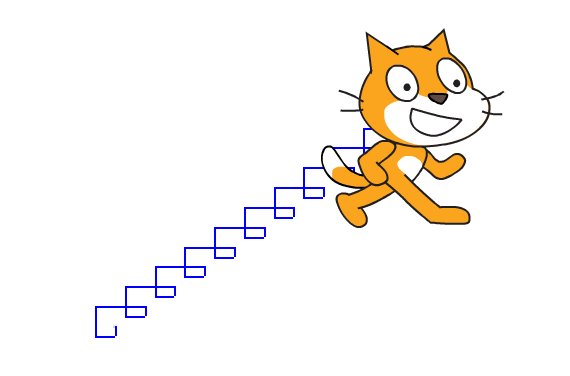
\includegraphics[scale=\scaleecran]{ecran-02-eg1}
\end{center}

On se place en $x=0$ et $y=0$ et on répète 10 fois les instructions suivantes :
\begin{itemize}
  \item s’orienter à $180$\textdegree
  \item avancer de $5$
  \item s’orienter à $-90$\textdegree 
  \item avancer de $10$
  \item s’orienter à $0$\textdegree
  \item avancer de $15$
  \item s’orienter à $90$\textdegree
  \item avancer de $25$
\end{itemize}

\bigskip

\textbf{Question.} À la fin, quelle est la valeur de $x$ ? 

%\begin{solution}
%Réponse : $x=150$, $y = 100$.
%\end{solution}

\end{enigme}



\begin{enigme}
On considère les instructions suivantes :
\begin{itemize}
  \item avancer de 20
  \item tourner vers la gauche de 15 degrés
\end{itemize}

\bigskip

\textbf{Question.} Combien de fois faut-il répéter ces deux instructions pour revenir à la position de départ ? 

%\begin{solution}
%Réponse : $360/15 = 24$ côtés.
%\end{solution}

\end{enigme}


\begin{enigme}
Le code suivant affiche un carré avec des petits triangles sur chaque côté. 

\bigskip

\textbf{Question.} Combien y a-t-il de petits triangles en tout ? 

\bigskip

\begin{center}
  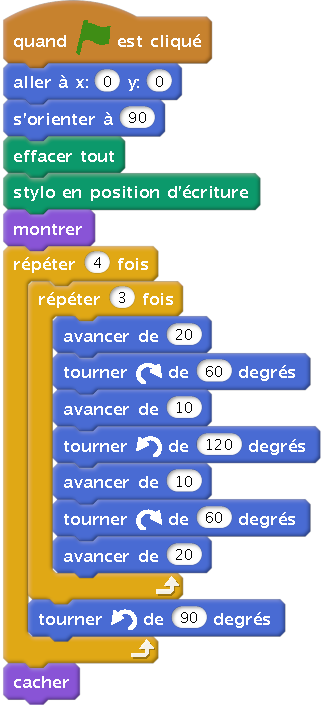
\includegraphics[scale=\scalebloc]{code-02-eg3}
\end{center} 

%\begin{solution}
%Réponse : $4 \times 3 = 12$ triangles.
%\end{solution}

\end{enigme}


\end{document}


